\subsection{$A$-膜与 $B$-膜}\label{flatcon}

这里我们将描述 $(B,A,A)$ 型膜的模空间的一些基本性质。除其他用途外，这将使我们更好地理解全纯极化在第 \ref{branecp} 节那样的论证中所起的作用。

首先考虑一个实辛流形 $S$ 的 $A$-模型，其辛形式为 $\omega$。秩 1 拉格朗日 $A$-膜 $\B$ 支撑在拉格朗日子流形 $L\subset S$ 上，并带有一个 $\CP$ 丛 $\L$，其联络 $\sA$ 与曲率 $\sF$ 满足 $\sF+\sB=0$。为形变 $\B$，一般可以同时形变 $L$ 与 $\sA$。$\sA$ 的一般形变具有形式 $\sA\to\sA+\veps\sa$，其中 $\sa$ 是一形式、$\veps$ 是小参数。为保持条件 $\sF+\sB=0$，要求 $\d\sa=0$。然而，若 $\sa$ 恰当，即 $\sa=\d\phi$（某个 $\phi$），则形变 $\sA\to\sA+\veps\sa$ 只是规范变换。因此非平凡形变由 de Rham 上同调 $H^1_{\dR}(L,\R)$ 给出。先假设 $L$ 紧。于是由 Hodge 理论，非平凡形变对应于调和一形式 $\sa$。

\begin{figure}[htbp]
 \centering
 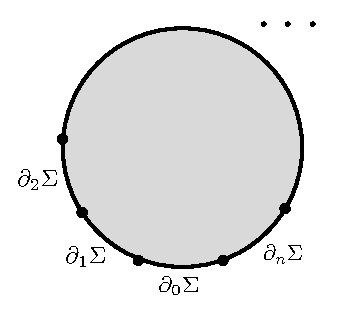
\includegraphics[width=0.42\textwidth]{figures/6.pdf}
 \caption{一个圆盘，其边界段依次标为 $\partial_0\Sigma$、$\partial_1\Sigma$、$\cdots$、$\partial_n\Sigma$。在每一段 $\partial_\alpha\Sigma$（$\alpha=0,1,\cdots,n$）上，边界条件由膜 $\B_\alpha$ 定义。顶点算符插入在各段之间的接点处。}\label{worldsheet}
\end{figure}

现在转而考虑 $L$ 的形变。局部可取坐标 $p_i,q^j$，使 $\omega=\sum_i\d p_i\d q^i$，且 $L$ 由 $p_1=\cdots=p_n=0$ 描述。任何一形式 $b=\sum_i b_i\d q^i$ 都给出 $L$ 的一个可能形变，其中方程 $p_i=0$ 被形变为 $p_i=\veps b_i$。这保持 $L$ 为拉格朗日子流形，当且仅当 $b$ 闭，即 $\d b=0$。然而，若 $b$ 恰当，$b=\d\rho$（某个函数 $\rho(q)$），则 $L$ 的形变由 $\rho$ 生成的 $M$ 的无穷小辛同胚给出，即
$\delta p_i=\{p_i,\rho\}=\partial\rho/\partial q^i$，
$\delta q_i=\{q_i,\rho\}=0$。用辛同胚对 $L$ 作形变，作为 $A$-膜 $\B$ 的形变是平凡的。稍后我们将明确演示这一点。因此在 $A$-模型中，$L$ 的非平凡形变在一阶对应于闭而非恰当的一形式，换言之对应于 de Rham 上同调 $H^1_{\dR}(L,\R)$。同样，若 $L$ 紧，这与调和一形式 $b$ 的空间相同。

比较上两段，我们看到 $\B$ 作为 $A$-膜的可能形变的模空间 $\M$ 上有一个明显的近复结构。在此近复结构中，$a+\i b$ 是 $(1,0)$ 型形变。事实上，这个近复结构可积，$\M$ 是复流形。

现在明确看看为什么一形式 $a$ 与 $b$ 中的恰当项代表 $\B$ 作为 $A$-膜的平凡形变。考虑定向二维流形 $\Sigma$ 上 $A$-模型的 $\sigma$-模型作用量，以及映射 $X:\Sigma\to M$。$\Sigma$ 的边界 $\partial\Sigma$ 是若干段 $\partial_\alpha\Sigma$ 的并，每段由带 $\CP$ 联络 $A_\alpha$ 的膜 $\B_\alpha$ 标记（图 \ref{worldsheet}）。设其中一段，比如 $\partial_0\Sigma$，由所关心的膜 $\B$ 标记，其 $\CP$ 联络为 $\sA$。在各段之间的接点处插入局部算符。设 $T$ 为这些接点的集合。$\sigma$-模型作用量的大部分是 $Q$-恰当的，其中 $Q$ 是通常的 $A$-模型微分。把非 $Q$-恰当的项写出，作用量可写成一般形式
\be\label{genformact} I=\int_\Sigma X^*(\omega)-\i\int_{\partial_0\Sigma}X^*(\sA)-\i\sum_{\alpha\ne0}\int_{\partial_\alpha\Sigma}X^*(\sA_\alpha)+\sum_{t\in T}c_t+\{Q,\cdots\}.\ee
非 $Q$-恰当的项是辛形式与 $\CP$ 联络的贡献，以及对应于接点处插入算符的可能端点贡献 $c_t$。$\partial_0\Sigma$ 的贡献在下文中很重要，故我们在 \eqref{genformact} 中把它单独分出。同样，重要的接点将是 $\partial_0\Sigma$ 的左右端点；我们称它们为 $t_r$ 与 $t_\ell$。若我们以 $a$ 或 $b$ 变分来形变膜 $\B$，即 $\delta\sA=a$，或 $\delta p_i=b_i,\ \delta q^j=0$，则作用量 $I$ 的改变是一个沿 $\partial_0\Sigma$ 的简单局部积分：
\be\label{varact}\delta I=-\i\int_{\partial_0\Sigma}(a_i+\i b_i)\d q^i.\ee
我们看到它自然地以组合 $a+\i b$ 依赖于 $a$ 与 $b$，这正是模空间 $\M$ 的复结构的表现。现在把它特殊化到我们将称为恰当变分的情形，即 $a+\i b=\d\nu$，其中 $\nu$ 是某个复值函数。此时积分化为边界项之和
\be\label{varacto}\delta I=-\i(\nu(t_r)-\nu(t_\ell))\ee
（我们简记 $\nu(X(t))$ 为 $\nu(t)$）。于是我们可以通过适当变换 $\partial_0\Sigma$ 端点处的插入来补偿恰当变分：
\be\label{endvar}\delta c_r=\i\nu(t_r),\quad\delta c_\ell=-\i\nu(t_\ell).\ee
最后，我们可以更精确地表述“由恰当形变联系的 $A$-膜等价”这一陈述。要断言 $\B$ 的恰当形变在某种意义下平凡，我们需要知道：在对 $\B$ 作恰当形变时，对于任何其他 $A$-膜 $\B'$，该如何处理 $\Hom(\B,\B')$ 与 $\Hom(\B',\B)$。式 \eqref{endvar} 回答了这个问题：它告诉我们，当对 $\B$ 作恰当形变以得到真正平凡的形变时，$\partial_0\Sigma$ 端点处的插入必须如何修改。

现在特殊化到辛流形 $S$ 实际上是复辛流形 $Y$、且 $\B$ 是 $(B,A,A)$ 型膜、支撑在复拉格朗日子流形 $L$ 上的情形。于是 $L$ 在某个复结构 $I$ 下是复流形，并且关于全纯辛形式 $\Omega=\omega_J+\i\omega_K$ 是拉格朗日的。为把 $\B$ 作为 $B$-膜形变，我们可以把 $L$ 作为复子流形形变，并把 $L$ 上的平坦 $\CP$ 丛 $\L$ 作为全纯线丛形变。$\B$ 的这两类形变都由复模参数化。若 $L$ 是紧 Kähler 流形，则无论把 $\B$ 视为 $I$ 型的 $B$-膜，还是视为关于 $\omega_J$ 或 $\omega_K$ 的 $A$-膜，参数化 $\B$ 形变的模空间 $\M$ 都相同。其理由本质上已在第 \ref{hyperm} 节解释：$\M$ 的切空间是 $(\B,\B)$ 系统的超对称基态空间，而后者可在物理 $\sigma$-模型层面定义，无需特殊化到某个扭转拓扑场论。然而，视我们把 $\M$ 视为复结构 $I$ 中 $B$-膜的模空间，还是视为辛结构 $\omega_J$ 或 $\omega_K$（或它们的线性组合）中 $A$-膜的模空间，$\M$ 具有不同的复结构。

在紧 Kähler 流形 $M$ 上，Hodge 分解把调和一形式表为 $(1,0)$ 型与 $(0,1)$ 型部分之和，给出展开 $a=a^{(1,0)}+a^{(0,1)}$、$b=b^{(1,0)}+b^{(0,1)}$。若把 $\M$ 视为参数化 $I$ 型 $B$-膜，则其复结构中的全纯方向由 $a^{(0,1)}$ 与 $b^{(1,0)}$ 参数化。若把它视为参数化关于辛结构 $\J_\zeta$ 的 $A$-膜，其中 $\J_\zeta$ 是 $\omega_J$ 与 $\omega_K$ 的线性组合，则全纯方向由
$a^{(0,1)}+\zeta b^{(0,1)}$ 与 $a^{(1,0)}-\zeta^{-1}b^{(0,1)}$ 参数化，其中 $\zeta$ 依赖于所考虑的线性组合（可选取约定使 $\zeta=1$ 对应 $\omega_J$、$\zeta=\i$ 对应 $\omega_K$）。当 $\zeta=0$ 时，$\J_\zeta$ 化为 $I$ 型 $B$-模型中适用的复结构；当 $\zeta=\infty$ 时，它化为相反的复结构，适用于 $-I$ 型 $B$-模型。

若 $L$ 不紧，则一般说来 $\B$ 作为 $B$-膜的模与作为 $A$-膜的模之间没有这种关系。与其一般地讨论，不如看看在我们的分析中实际重要的例子会怎样。这就是 $(B,A,A)$ 型膜 $\F$ 支撑在全纯极化 $\varPi$ 的一个叶 $F$ 上、且 $\CP$ 丛平凡的情形。由于 $F\cong\C^n$，$F$ 单连通，$\F$ 作为 $A$-膜实际上没有模。另一方面，$\F$ 作为 $B$-膜确有模，因为 $\varPi$ 的不同叶支撑不等价的 $B$-膜。局部可用全纯变量 $q^i$ 参数化叶的选择，用全纯变量 $p_i$ 参数化叶，使 $\Omega=\sum_i\d p_i\d q^i$。于是特定的叶由指定 $q^i$ 的值确定，比如 $q^i=w^i$。不同的 $w^i$ 选择标记不同的 $B$-膜；但粗略地说——稍后我们会给出更准确的说法——这些膜作为 $A$-膜全都相同。

“由给定 $\vec w=(w^1,w^2,\cdots,w^n)$ 标记的 $A$-膜 $\F$ 与 $\vec w$ 无关”这一断言可能显得费解，因为对 $\vec w$ 的依赖在我们的分析中其实很重要。关键在于，我们总是把膜 $\F$ 与 $\Hom(\B_\cc,\F)$ 中一个 distinguished 元素一起考虑，该元素对应于波函数 $\alpha=(\d\vec p)^{1/2}$。膜 $\F$ 连同 $\Hom(\B_\cc,\F)$ 的这个特定元素，确实非平凡地——而且正如我们将看到的，全纯地——依赖于 $\vec w$。要得到 $\F$ 的平凡变分，我们希望把 $\F$ 的改变与端点耦合 $c_\ell,c_r$ 的改变（如式 \eqref{endvar} 所示）配套。这与使用不依赖 $\vec w$ 的波函数 $\alpha=(\d\vec p)^{1/2}$ 不同。

让我们看看，当我们把膜 $\F$ 变到同一全纯极化的邻近叶，例如把 $w^i$ 平移某些复常数 $b^i$ 时，情形如何。回顾在量子化相关的情形中，复化辛形式为 $\omega_\C=-\i\Omega$，且 $\F$ 的 $\CP$ 丛平凡。作用量（见式 \eqref{genformact} 与 \eqref{toldo}）变为
\be\label{specformact} I=-\i\int_\Sigma X^*(\Omega)+c_\ell+c_r+\cdots+\{Q,\cdots\},\ee
其中我们省略了区间 $\partial_0\Sigma$ 之外的边界项与耦合，因为它们不受我们即将所作的形变影响。为描述通过改变 $\vec w$ 对膜 $\F$ 所作的改变，我们在 $\partial_0\Sigma$ 附近变分映射 $X$：$\delta p_i=0$、$\delta q^i=b^i$。由 $\Omega=\sum_i\d p_i\d q^i$，得到
\be\label{acttrans}\delta I=\i\int_{\partial_0\Sigma}b^i\d p_i=\i b^i p_i(t_r)-\i b^i p_i(t_\ell).\ee
于是为得到真正平凡的形变，补偿性的端点变分为
\be\label{nactra}\delta c_r=\i b^i p_i(t_r),\quad\delta c_\ell=-\i b^i p_i(t_\ell).\ee

我们可以如下解释这些结果。首先，$\F$ 的这个变分是全纯的，因为作用量的变分正比于 $\delta w^i=b^i$，而不含正比于 $\delta\bar{w^i}=\bar{b^i}$ 的项。这证实了第 \ref{branecp} 节中的断言。其次，为补偿 $\F$ 的位移所需的特定变分 $\delta c_\ell$、$\delta c_r$，可以直观地理解如下。$\F$ 的位移由 $b^i\frac{\partial}{\partial q^i}$ 给出，它生成 $q^i\to q^i+b^i$。量子力学上，$b^i\frac{\partial}{\partial q^i}$ 对应于 $\i b^i p_i$。对于表示 $\Hom(\B',\F)$ 或 $\Hom(\F,\B')$（$\B'$ 为某个其他膜）中元素的顶点算符，其修正涉及乘以 $\pm\i b^i p_i$。

$b^i p_i$ 如何作用在 $\Hom(\B',\F)$ 或 $\Hom(\F,\B')$ 上，取决于所考虑的膜的类型。设 $\B'=\B_\cc$。则 $\Hom(\B_\cc,\F)$ 与 $\Hom(\F,\B_\cc)$ 等同于 $H^0(F,K_F^{1/2})$。一般元素形如 $f(\vec p)(\d\vec p)^{1/2}$，而 $b^i p_i$ 作为乘法算符作用。另一方面，设 $\B'$ 是拉格朗日 $A$-膜，其支撑 $L$ 与 $F$ 交于单点 $w$。则作用在 $\Hom(\F,\B')$ 或 $\Hom(\B',\F)$ 上时，$p_i$ 可用其在 $w$ 处的值代替。

最后，考虑当我们变分全纯极化 $\varPi$ 的叶时会发生什么。$\varPi$ 的邻近叶等价，条件是我们按 $\delta q^i=b^i$ 改变叶时，如上所述用 $\pm\i b^i p_i$ 变换 $\Hom(\F,\B')$ 与 $\Hom(\B',\F)$。这可以看作由 $W$ 参数化的膜族上的平坦联络。但它是不可积的平坦联络。为积分这个平坦联络，我们必须把作用在 $\F$ 与其他膜之间角上的算符 $\pm\i b^i p_i$ 取指数。例如，要断言 $q^i$ 相差非无穷小平移 $b^i$ 的两个纤维等价，我们必须把它们与 $\B_\cc$ 的角乘以 $\exp(\pm\i\sum_i b^i p_i)$。这样的指数函数是不允许的；我们只允许 $p$ 的多项式函数。无法积分这个平坦联络是一个特性，而不是缺陷。在我们的应用中，断言 $\varPi$ 的不同纤维等价并不自然。
